% Copyright 2020 by Robert Hildebrand
%This work is licensed under a
%Creative Commons Attribution-ShareAlike 4.0 International License (CC BY-SA 4.0)
%See http://creativecommons.org/licenses/by-sa/4.0/% 



%\documentclass[../open-optimization/open-optimization.tex]{subfiles}
% 
%\begin{document}

\chapter{Integer Programming Formulations}
\label{sec:IP-formulations} 
\begin{outcome}
\begin{enumerate}
\item[A.] Learn classic integer programming formulations.
\item[B.] Demonstrate different uses of binary and integer variables.
\item[C.]  Demonstrate the format for modeling an optimization problem with sets, parameters, variables, and the model.
\end{enumerate}
\end{outcome}
%\begin{comment}
%We will learn about complexity theory in a subsequent section.  But take note of the complexity classification of each problem ( \polynomial,\npcomplete, \nphard) to get a sense of how difficult the problem is.  We will define these terms later.
%\end{comment}


\begin{resource}
\begin{itemize}
\item The AIMMS modeling has many great examples.  It can be book found here:\href{https://www.aimms.com/english/developers/resources/manuals/optimization-modeling}{AIMMS Modeling Book}.
\item \href{http://web.mit.edu/15.053/www/AMP-Chapter-09.pdf}{MIT Open Courseware}
\item  For many real world examples, see this book \href{https://link-springer-com.ezproxy.lib.vt.edu/book/10.1007/978-1-4939-1007-6}{
Case Studies in Operations Research
Applications of Optimal Decision Making, edited by  Murty, Katta G}.
Or find it \href{https://www.springer.com/gp/book/9781493910069}{here}.
\item \href{https://github.com/Gurobi/modeling-examples}{GUROBI modeling examples by GUROBI}
\item \href{https://github.com/open-optimization/open-optimization-or-examples/tree/master/integer-programming}{GUROBI modeling examples by Open Optimization that are linked in this book}
\end{itemize}

\end{resource}

In this section, we will describe classical integer programming formulations.     These formulations may reflect  a real world problem exactly, or may be part of the setup of a real world problem.   

\section{Knapsack Problem}
The \emph{knapsack problem}\footnote{\href{https://www.youtube.com/watch?v=GteOoMGUOdY}{Video! - Michel Belaire (EPFL) teaching knapsack problem}} can take different forms depending on if the variables are binary or integer.  The binary version means that there is only one item of each item type that can be taken.  This is typically illustrated as a backpack (knapsack) and some items to put into it (see  \autoref{fig:wiki/File/knapsack}), but has applications in many contexts.  



 \includefigurestatic[Knapsack Problem: which items should we choose take in the knapsack that maximizes the value while respecting the 15kg weight limit?][width=.4\linewidth][h]{wiki/File/knapsack}

\begin{general}{Binary Knapsack Problem}{\npcomplete}
Given an non-negative weight vector $a \in \Q^n_+$, a capacity $b \in \Q_+$, and objective coefficients $c \in \Q^n$, 
\begin{equation}
\begin{split}
\max \ \ & c^\top x\\
\text{s.t.}\ \ & a^\top x \leq b\\
& x \in \{0,1\}^n
\end{split}
\end{equation}
\end{general}
 


 
%\begin{figure}[H]
%\begin{center}
%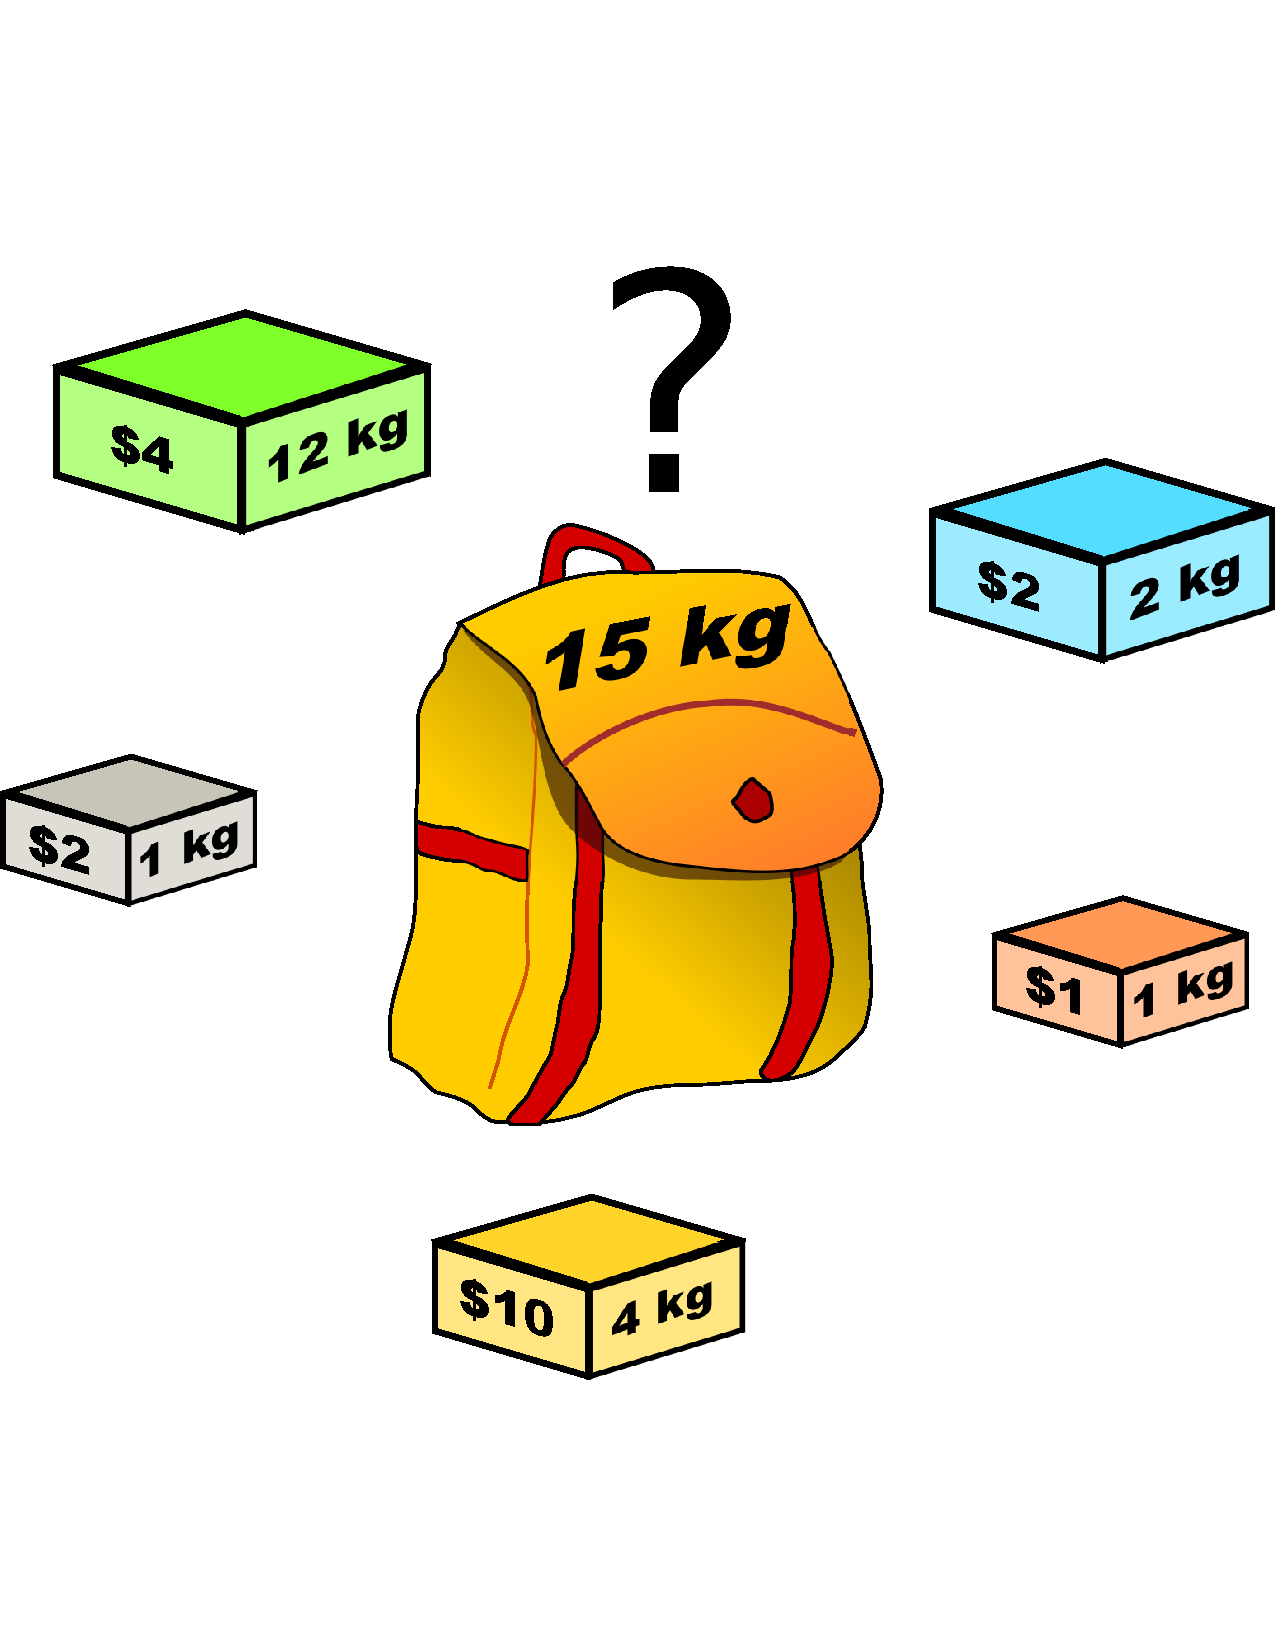
\includegraphics[scale = 0.2]{knapsack}\footnotemark 
%\end{center}
%\label{fig:knapsack}
%\caption{Knapsack Problem: which items should we choose take in the knapsack that maximizes the value while respecting the 15kg weight limit?}
%\end{figure}
%\footnotetext{\url{https://en.wikipedia.org/wiki/Knapsack_problem}}

\begin{examplewithcode}{Knapsack}{https://github.com/open-optimization/open-optimization-or-examples/blob/master/integer-programming/knapsack-problem.ipynb}
\label{example:knapsack}
You have a knapsack (bag) that can only hold W = 15 kgs.  There are 5 items that you could possibly put into your knapsack.  The items (weight, value) are given as:
(12 kg, $\$$4), (2 kg, $\$$2), (1kg, $\$$2), (1kg, $\$$1), (4kg, $\$$10).  Which items should you take to maximize your value in the knapsack? See \autoref{fig:wiki/File/knapsack}.\\

\noindent \textbf{Variables:}
\begin{itemize}
\item let $x_i = 0$ if item $i$ is in the bag
\item let $x_i = 1$ if item $i$ is not in the bag
\end{itemize}
\textbf{Model:}
\begin{align}
\max  \  \ &4 x_1 + 2 x_2 + 2 x_3 + 1 x_4 + 10 x_5 \tag{Total value}\\
\text{ s.t. }\ \ &  12 x_1 + 2 x_2 + 1 x_3 + 1 x_4 + 4 x_5 \leq 15 \tag{Capacity bound}\\
& x_i \in \{0,1\} \text{ for } i=1, \dots, 5 \tag{Item taken or not}
\end{align}
\end{examplewithcode}
In the integer case, we typically require the variables to be non-negative integers, hence we use the notation $x \in \Z^n_+$.  This setting reflects the fact that instead of single individual items, you have item types of which you can take as many of each type as you like that meets the constraint.
\begin{general}{Integer Knapsack Problem}{\npcomplete}
Given an non-negative weight vector $a \in \Q^n_+$, a capacity $b \in \Q_+$, and objective coefficients $c \in \Q^n$, 
\begin{equation}
\begin{split}
\max \ \ & c^\top x\\
\text{s.t.}\ \ & a^\top x \leq b\\
& x \in \Z^n_+
\end{split}
\end{equation}
\end{general}
We can also consider an equality constrained version
\begin{general}{Equality Constrained Integer Knapsack Problem}{\nphard}
Given an non-negative weight vector $a \in \Q^n_+$, a capacity $b \in \Q_+$, and objective coefficients $c \in \Q^n$, 
\begin{align}
\max \ \ & c^\top x\\
\text{s.t.}\ \ & a^\top x = b\\
& x \in \Z^n_+
\end{align}
\end{general}
\begin{example}
\label{ex:min-coins}
Using pennies, nickels, dimes, and quarters, how can you minimize the number of coins you need to to make up a sum of $83\cent$? 

\textbf{Variables:}
\begin{itemize}
\item Let $p$ be the number of pennies used
\item Let $n$ be the number of nickels used
\item Let $d$ be the number of dimes used
\item Let $q$ be the number of quarters used
\end{itemize}
\textbf{Model}
\begin{align*}
\min \quad & p + n + d + q & \text{ total number of coins used}\\
\text{ s.t. } \quad & p + 5n + 10d + 25 q = 83 & \text{sums to } 83 \cent\\
& p,d,n,q \in \Z_+ & \text{each is a non-negative integer}
\end{align*}
\end{example}
\section{Capital Budgeting}


% Copywrite Robert Hildeband 2019


	\textcolor{blue}{A firm has $n$ projects it could undertake to maximize revenue, but budget limitations require that not all can be completed.}\\
	\textcolor{blue}{Project $j$ expects to produce revenue $c_j$\\
		Project $j$ requires investment $a_{ij}$ in time period $i$ for $i = 1,\ldots,m$\\
		In time period $i$, capital $b_i$ is available}
		
		Let $x_i$ be a binary variable such that $x_i = 1$ if we choose investment $i$ and $x_i = 0$ otherwise.  The the model can be given as:
	\begin{align*}
	\max ~~~& \sum_{j = 1}^n c_jx_j\\
	s.t. ~~~&\sum_{j = 1}^n a_{ij}x_j\leq b_i, ~~~i = 1,\ldots m\\
	& x_j \in \{0,1\} , \ j = 1,\ldots,n
	\end{align*}


Consider the example given in the following table.
	\begin{table}[h]
		\centering
		\resizebox{\columnwidth}{!}{%
			\begin{tabular}{|c|c|c|c|}%[<+->]
				\hline
				Project & $\mathbb{E}$[Revenue] & Resources required in week 1 & Resources required in week 2\\\hline
				\rowcolor{gray!10} 1 & 10 & 3 & 4\\
				\hline
				2 & 8 & 1 & 2\\\hline
				\rowcolor{gray!10} 3 & 6 & 2 & 1\\
				\hline
				Resources available & & 5 & 6\\
				\hline
		\end{tabular}}
	\end{table}
	$$
	\max~~~~~ 10x_1+8x_2+6x_3
	$$
	subject to
	\begin{align*}
	3x_1+1x_2+2x_3\leq5\\
	4x_1+2x_2+1x_3\leq6\\
	x_j \in \{0,1\},\  j = 1,2,3
	\end{align*}



\section{Set Covering}
\begin{resource}
\href{https://www.youtube.com/watch?v=cjSeHSjPmsk}{Video! - Michel Belaire (EPFL) explaining set covering problem}
\end{resource}

The \emph{set covering} problem can be used for a wide array of problems.    We will see several examples in this section.

\begin{general}{Set Covering}{\npcomplete}
\label{general:set-covering}
Given a set $V$ with subsets $V_1, \dots, V_l$, determine the smallest subset $S \subseteq V$ such that 
$S \cap V_i \neq \emptyset$ for all $i=1, \dots, l$.

The set cover problem can be modeled as
\begin{equation}
\begin{split}
\min \ \ & \one^\top x\\
\text{s.t.} \ \ & \sum_{v \in V_i} x_v \geq 1 \text{ for all } i =1, \dots, l \\ 
& x_v \in \{0,1\} \text{ for all } v \in V
\end{split}
\end{equation}
where $x_v$ is a 0/1 variable that takes the value $1$ if we include item $j$ in set $S$ and $0$ if we do not include it in the set $S$.  
\end{general}

\begin{resource}
See \href{https://download.aimms.com/aimms/download/manuals/AIMMS3OM_MediaSelection.pdf}{AIMMS - Media Selection} for an example of set covering applied to media selection.
\end{resource}

\todo[inline]{
Add flight crew scheduling example and images.
}

One specific type of set cover problem is the \emph{vertex cover} problem.
\begin{general}{Example: Vertex Cover}{\npcomplete}
Given a graph $G = (V,E)$ of vertices and edges, we want to find a smallest size subset $S \subseteq V$ such that every for every $e = (v,u) \in E$, either $u$ or $v$ is in $S$.   

We can write this as a mathematical program in the form:
\begin{equation}
\begin{split}
\min \ \ & \one^\top x\\
\text{s.t.} \ \ & x_u + x_v \geq 1 \text{ for all } (u,v) \in E \\ 
& x_v \in \{0,1\} \text{ for all } v \in V.
\end{split}
\end{equation}
\end{general}




\begin{examplewithcode}{Set cover: Fire station placement}{https://github.com/open-optimization/open-optimization-or-examples/blob/master/integer-programming/fire-station-covering.ipynb}
\label{example:fire-station}

In the fire station problem, we seek to choose locations for fire stations such that any district either contains a fire station, or neighbors a district that constains a fire station.  Figure~\ref{fig:tikz/Illustration1.pdf} depicts the set of districts and an example placement of locations of fire stations.  How can we minimize the the total number of fire stations that we need?


\noindent \textbf{Sets:}
\begin{itemize}
\item Let $V$ be the set of districts ($V = \{1, \dots, 16\}$)
\item Let $V_i$ be the set of districts that neighbor district $i$ (e.g. $V_1 = \{2,4,5\}$).
\end{itemize}

\noindent \textbf{Variables:}
\begin{itemize}
\item let $x_i = 1$ if district $i$ is chosen to have a fire station.
\item let $x_i = 0$ otherwise.
\end{itemize}
\textbf{Model:}
\begin{align}
\min  \  \ &\sum_{i \in V} x_i \tag{ \# \text{ open fire stations}}\\
\text{ s.t. }\ \ &  x_i + \sum_{j \in V_i} x_j \geq 1 & \forall{i \in V} \tag{Station proximity requirement}\\
& x_i \in \{0,1\} & \text{ for } i\in V  \tag{station either open or closed}
\end{align}
\end{examplewithcode}

\includefiguresource[Layout of districts and possible locations of fire stations.][][h]{tikz/Illustration1.pdf}
\includefiguresource[Set cover representation of fire station problem.  For example, choosing district 16 to have a fire station covers districts 13, 15, and 16.]{tikz/Illustration2.pdf}
\includefiguresource[Graph representation of fire station problem.  Every node is connected to a chosen node by an edge]{tikz/Illustration3.pdf}



%\documentclass[../open-optimization/open-optimization.tex]{subfiles}

%%%%%%%%%
%\begin{document}
%%%%%%%%%

\begin{general}{Set Covering - Matrix description}{\npcomplete}
\label{general:set-covering-alternate}
Given a non-negative matrix $A \in \{0,1\}^{m \times n}$, a non-negative vector, and an objective vector $c \in \R^n$, the set cover problem is
\begin{equation}
\begin{split}
\max \ \ & c^\top x\\
\text{s.t.}. \ \ & Ax \geq \one \\
& x \in \{0,1\}^n.
\end{split}
\end{equation}
\end{general}
\begin{examplewithoutcode}{Vertex Cover with matrix}{code:vertex-cover-matrix}
An alternate way to solve \nameref{ex:vertex-cover} is to define the \emph{adjacency matrix} $A$ of the graph.  The adjacency matrix is a $|E| \times |V|$ matrix with $\{0,1\}$ entries.  The each row corresponds to an edge $e$ and each column corresponds to a node $v$.  For an edge $e = (u,v)$, the corresponding row has a $1$ in columns corresponding to the nodes $u$ and $v$, and a 0 everywhere else.  Hence, there are exactly two 1's per row.  Applying the formulation above in \nameref{general:set-covering-alternate} models the problem.
\end{examplewithoutcode}




%%%%%%%%%
%\end{document}
%%%%%%%%%




\subsection{Covering (Generalizing Set Cover)}
We could also allow for a more general type of set covering where we have non-negative integer variables and a right hand side that has values other than $1$.
\begin{general}{Covering}{\npcomplete}
\label{general:covering}
Given a non-negative matrix $A \in \Z_+^{m \times n}$, a non-negative vector $b \in \Z^m$, and an objective vector $c \in \R^n$, the set cover problem is
\begin{equation}
\begin{split}
\max \ \ & c^\top x\\
\text{s.t.}. \ \ & Ax \geq b \\
& x \in\Z^n_+.
\end{split}
\end{equation}
\end{general}

%\todo[inline]{
% Add Nurse scheduling problem.
%}
%
%\begin{examplewithcode}{Nurse Scheduling}{code:nurse-scheduling}
%Suppose that we have $n$ full-time nurses employed and $p$ part-time nurses employed.  We need to schedule nurses such that, for each day of the week, we have enough nurses on hand to cover all the tasks.  
%
%\todo[inline]{Add complete example}
%\end{examplewithcode}




\section{Assignment Problem}

The \emph{assignment problem} (machine/person to job/task assignment) seeks to assign tasks to machines in a way that is most efficient.   This problem can be thought of as having a set of machines that can complete various tasks (textile machines that can make t-shirts, pants, socks, etc) that require different amounts of time to complete each task, and given a demand, you need to decide how to alloacte your machines to tasks.

Alternatively, you could be an employer with a set of jobs to complete and a list of employees to assign to these jobs.  Each employee has various abilities, and hence, can complete jobs in differing amounts of time.  And each employee's time might cost a different amout.  How should you assign your employees to jobs in order to minimize your total costs?


\begin{general}{Assignment Problem}{}{}
Given $m$ machines and $n$ jobs, find a least cost assignment of jobs to machines. The cost of assigning job $j$ to machine $i$ is $c_{ij}$.
\end{general}

\todo[inline]{
Include picture and example data
}


\begin{examplewithcode}{Machine Assignment}{https://github.com/open-optimization/open-optimization-or-examples/blob/master/integer-programming/assignment-problem.ipynb}
\noindent \textbf{Sets:}
\begin{itemize}
\item Let $I = \{0,1,2,3\}$ set of machines.
\item Let $J = \{0,1, 2,3\}$ be the set of tasks.
\end{itemize}

\noindent \textbf{Parameters:}
\begin{itemize}
\item $c_{ij}$ - the cost of assigning machine $i$ to job $j$
%\item $c_j$ is given in column "$\mathbb{E}$[Revenue]".
%\item $b_i$ is given in row "Resources available".
%\item $a_{ij}$ given in row $j$, and column for week $i$.
\end{itemize}

\noindent \textbf{Variables:}
\begin{itemize}
\item Let 
\begin{equation*}
x_{ij} = \begin{cases}
1 & \text{if machine $i$ assigned to job $j$}\\
0 & \text{otherwise.}
\end{cases}
\end{equation*}
%\item let $x_i = 1$ if investment $i$ is not chosen
\end{itemize}

\noindent  \textbf{Model:}
\begin{align*}
	\min\ \ \  & \sum_{i \in I, j \in J} c_{ij} x_{ij} \tag{Minimize cost}\\
	s.t. \ \ & \sum_{i \in I} x_{ij} = 1 & \text{for all $j \in J$}
	 \tag{All jobs are assigned one machine}\\
	& \sum_{j \in J} x_{ij} = 1 & \text{for all $i\in I$}
	 \tag{All machines are assigned to a job}\\
	 & x_{ij} \in \{0,1\} \forall i \in I, j \in J
	  \end{align*}
\end{examplewithcode}



\section{Facility Location}
\begin{resource}{}{}
\begin{itemize}
\item \href{https://en.wikipedia.org/wiki/Facility_location_problem}{Wikipedia - Facility Location Problem}
\item See \href{https://github.com/Gurobi/modeling-examples/tree/master/facility_location}{GUROBI Modeling Examples - Facility Location}.
\end{itemize}
\end{resource}
The basic model of the facility location problem is to determine where to place your stores or facilities in order to be close to all of your customers and hence reduce the costs transportation to your customers.  Each customer is known to have a certain demand for a product, and each facility has a capacity on how much of that demand it can satisfy.  Furthermore, we need to consider the cost of building the facility in a given location.

This basic framework can be applied in many types of problems and there are a number of variants to this problem.   We will address two variants: the \emph{capacitated facility location problem} and the \emph{uncapacitated facility location problem}.  
%\todo[inline]{
%Add discussion on Facility Location Problems and pictures.
%}



\subsection{Capacitated Facility Location}

\begin{general}{Capacitated Facility Location}{\npcomplete}
Given costs connections $c_{ij}$ and fixed building costs $f_i$, demands $d_j$ and capacities $u_i$, the capacitated facility location problem is 

\noindent \textbf{Sets:}
\begin{itemize}
\item Let $I = \{1,\dots, n\}$ be the set of facilities.
\item Let $J = \{1, \dots, m\}$ be the set of customers.
\end{itemize}

\noindent \textbf{Parameters:}
\begin{itemize}
\item $f_i$ - the cost of opening facility $i$.
\item $c_{ij}$ - the cost of fulfilling the complete demand of customer $j$ from facility $i$.
\item $u_{i}$ - the capacity of facility $i$.
\item $d_{j}$ - the demand by customer $j$.
%\item $c_j$ is given in column "$\mathbb{E}$[Revenue]".
%\item $b_i$ is given in row "Resources available".
%\item $a_{ij}$ given in row $j$, and column for week $i$.
\end{itemize}

\noindent \textbf{Variables:}
\begin{itemize}
\item Let 
\begin{equation*}
x_{i} = \begin{cases}
1 & \text{if we open facility $i$,}\\
0 & \text{otherwise.}
\end{cases}
\end{equation*}
\item Let $y_{ij} \geq 0$ be the fraction of demand of customer $j$ satisfied by facility $i$.
%\item let $x_i = 1$ if investment $i$ is not chosen
\end{itemize}

\noindent  \textbf{Model:}
\begin{align}
\min & \displaystyle\sum_{i=1}^n\sum_{j=1}^mc_{ij}y_{ij}+\sum_{i=1}^nf_ix_i \tag{total cost}\\
\text{s.t.} & \displaystyle\sum_{i=1}^ny_{ij}=1 \text{ for all }j=1,\dots,m \tag{assign demand to facility}\\
& \displaystyle \sum_{j=1}^md_jy_{ij}\leqslant u_ix_i\text{ for all }i=1\dots,n \tag{capacity of facility $i$}\\
&y_{ij}\geqslant0\text{ for all }i=1,\dots,n \text{ and }j=1,\dots,m \tag{nonnegative fraction of demand satisfied}\\
&x_i\in\{0,1\}\text{ for all } i=1,\dots,n \tag{open/not open facility}
\end{align}

\end{general}

\subsection{Uncapacitated Facility Location}

\begin{general}{Uncapacitated Facility Location}{\npcomplete}
Given costs connections $c_{ij}$ and fixed building costs $f_i$, the uncapacitated facility location problem is 
\begin{equation}
\begin{array}{rl}
\min & \displaystyle\sum_{i=1}^n\sum_{j=1}^mc_{ij}z_{ij}+\sum_{i=1}^nf_ix_i \\
\text{s.t.} & \displaystyle\sum_{i=1}^nz_{ij}=1 \text{ for all }j=1,\dots,m \\
& \displaystyle \sum_{j=1}^mz_{ij}\leqslant Mx_i\text{ for all }i=1\dots,n \\
&z_{ij}\in\{0,1\}\text{ for all }i=1,\dots,n \text{ and }j=1,\dots,m\\
&x_i\in\{0,1\}\text{ for all } i=1,\dots,n
\end{array}
\end{equation}
Here $M$ is a large number and can be chosen as $M = m$, but could be refined smaller if more context is known.
\end{general}


\section{Basic Modeling Tricks - Using Binary Variables}
\begin{resource}
\begin{itemize}
\item \href{https://jump.dev/JuMP.jl/stable/tutorials/linear/tips_and_tricks/}{JuMP tips and tricks}
\item \href{https://docs.mosek.com/modeling-cookbook/mio.html}{Mosek Modeling Cookbook}
\end{itemize}
\end{resource}
In this section, we describe ways to model a variety of constraints that commonly appear in practice.  The goal is changing constraints described in words to constraints defined by math.

Binary variables can allow you to model many types of constraints.  We discuss here varios logical constraints where we assume that $x_i \in \{0,1\}$ for $i=1, \dots, n$.  We will take the meaning of the variable to be selecting an item.

\begin{enumerate}
 \item If item $i$ is selected, then item $j$ is also selected.
 \begin{equation}
 x_i \leq x_j
 \end{equation}
 \begin{enumerate}
 \item If any of items $1, \dots, 5$ are selected, then item $6$ is selected.
 \begin{equation}
 x_1 + x_2 + \dots + x_5 \leq 5 \cdot x_6
 \end{equation}
 Alternatively!
 \begin{equation}
 x_i \leq x_6 \ \ \ \ \text{ for all } i=1, \dots, 5
 \end{equation}
 \end{enumerate}
 \item If item $j$ is not selected, then item $i$ is not selected.
 \begin{equation}
x_i \leq x_j
 \end{equation}
  \begin{enumerate}
 \item If item $j$ is not selected, then all items $1, \dots, i$ are not selected.
 \begin{equation}
 x_1 + x_2 + \dots + x_i \leq i \cdot x_j
 \end{equation}
 \end{enumerate}
  \item If item $j$ is not selected, then item $i$ is not selected.
 \begin{equation}
x_i \leq x_j
 \end{equation}
\item Either item $i$ is selected or item $j$ is selected, but not both.
 \begin{equation}
 x_i + x_j = 1
 \end{equation}
\item Item $i$ is selected or item $j$ is selected or both.
 \begin{equation}
 x_i + x_j \geq 1
 \end{equation}
\item If item $i$ is selected, then item $j$ is not selected.
 \begin{equation}
x_j \leq (1-x_i)
 \end{equation}

\item At most one of items $i ,j$, and $k$ are selected.
 \begin{equation}
 x_i + x_j + x_k \leq 1
 \end{equation}
\item At most two of items $i,j,$ and $k$ are selected.
 \begin{equation}
 x_i + x_j + x_k \leq 2
 \end{equation}
\item Exactly one of items $i,j,$ and $k$ are selected.
 \begin{equation}
  x_i + x_j + x_k = 1
 \end{equation}
\end{enumerate}

These tricks can be connected to create different function values.  

\begin{example}{Variable takes one of three values}{}
Suppose that the variable $x$ should take one of the three values $\{4, 8, 13\}$. This can be modeled using three binary variables as
\begin{align*}
x=4z_1 +8z_2 +13z_3\\
 z_1 +z_2 +z_3 =1\\
z_i \in \{0, 1\} \text{ for } i = 1, 2,3.
\end{align*}
As a convenient addition, if we want to add the possibility that it takes the value $0$, then we can model this as 
\begin{align*}
x=4z_1 +8z_2 +13z_3\\
 z_1 +z_2 +z_3 \leq 1\\
z_i \in \{0, 1\} \text{ for } i = 1, 2,3.
\end{align*}
\end{example}


We can also model variable increases at different amounts.  \begin{example}{Discount for buying more}{}
Suppose you can choose to buy 1, 2, or 3 units of a product, each with a decreasing cost.  The first unit is \$10, the second is \$5, and the third unit is \$3.
\begin{align*}
x=10z_1 +5z_2 +3z_3\\
 z_1\geq z_2 \geq z_3\\
z_i \in \{0, 1\} \text{ for } i = 1, 2,3.
\end{align*}
Here, $z_i$ represents if we buy the $i$th unit.  The inequality constraints impose that if we buy unit $j$, then we must by all units $i$ with $i < j$.
\end{example}


\subsection{Connecting to continuous variables}

Let $x_i \geq 0$ and $y_i \in \{0,1\}$ for all $i=1, \dots, n$.

\begin{enumerate}
\item If $x_i > 0$, then $y_i = 1$.
\begin{equation}
x_i \leq M y_i
\end{equation}
where $M$ is a suffiently large upper bound on the variable $x_i$.
\item If $x_i = 0$, then $y_i = 0$.\\
This is harder to model!  Alternatively, we try modeling "if $x_i$ is sufficiently small, then $y_i = 0$.   For instance, if $x_i \leq 0.0000001$, then $y_i = 0$.
This can be modeled as
\begin{equation}
x_i - 0.0000001 \geq y_i -1.
\end{equation}
\item If $y_i = 1$, then $x_i \geq 5$
\begin{equation}
5y_i \leq x_i.
\end{equation}


\subsection{Exact absolute value}
% Borrowed from Mosek Cookbook
Suppose we need to model an exact equality
$$
|x|=t
$$
It defines a non-convex set, hence it is not conic representable. If we split $x$ into positive and negative part $x=x^{+}-x^{-}$, where $x^{+}, x^{-} \geq 0$, then $|x|=x^{+}+x^{-}$as long as either $x^{+}=0$ or $x^{-}=0$. That last alternative can be modeled with a binary variable, and we get a model of  :
$$
\begin{aligned}
x &=x^{+}-x^{-} \\
t &=x^{+}+x^{-} \\
0 & \leq x^{+}, x^{-} \\
x^{+} & \leq M z \\
x^{-} & \leq M(1-z) \\
z & \in\{0,1\}
\end{aligned}
$$
where the constant $M$ is an a priori known upper bound on $|x|$ in the problem.

\subsubsection{Exact 1 -norm}
We can use the technique above to model the exact $\ell_{1}$-norm equality constraint
$$
\sum_{i=1}^{n}\left|x_{i}\right|=c
$$
where $x \in \mathbb{R}^{n}$ is a decision variable and $c$ is a constant. Such constraints arise for instance in fully invested portfolio optimizations scenarios (with short-selling). As before, we split $x$ into a positive and negative part, using a sequence of binary variables to guarantee that at most one of them is nonzero:
$$
\begin{aligned}
x &=x^{+}-x^{-} \\
0 & \leq x^{+}, x^{-}, \\
x^{+} & \leq c z \\
x^{-} & \leq c(e-z), \\
\sum_{i} x_{i}^{+}+\sum_{i} x_{i}^{-} &=c, \\
z & \in\{0,1\}^{n}, x^{+}, x^{-} \in \mathbb{R}^{n}
\end{aligned}
$$

\subsubsection{Maximum}
The exact equality $t=\max \left\{x_{1}, \ldots, x_{n}\right\}$ can be expressed by introducing a sequence of mutually exclusive indicator variables $z_{1}, \ldots, z_{n}$, with the intention that $z_{i}=1$ picks the variable $x_{i}$ which actually achieves maximum. Choosing a safe bound $M$ we get a model:
$$
\begin{aligned}
x_{i} & \leq t \leq x_{i}+M\left(1-z_{i}\right), i=1, \ldots, n \\
z_{1}+\cdots+z_{n} &=1, \\
z & \in\{0,1\}^{n}
\end{aligned}
$$









\section{Network Flow}
\todo[inline]{Fix up this section}
\begin{center}
\href{https://pixabay.com/illustrations/under-construction-construction-sign-2408060/}{
\includegraphics[scale = 0.05]{optimization/figures/under-construction-2408060_1280}}
\end{center}
\subsection{Example - Multicommodity Flow}

\url{https://en.wikipedia.org/wiki/Multi-commodity_flow_problem}
The \textbf{multi-commodity flow problem} is a
\href{flow_network}{network flow} problem with multiple commodities
(flow demands) between different source and sink nodes.

\paragraph{Problem Definition}

Given a flow network \(\,G(V,E)\), where edge \((u,v) \in E\) has
capacity \(\,c(u,v)\). There are \(\,k\) commodities
\(K_1,K_2,\dots,K_k\), defined by \(\,K_i=(s_i,t_i,d_i)\), where
\(\,s_i\) and \(\,t_i\) is the \textbf{source} and \textbf{sink} of
commodity \(\,i\), and \(\,d_i\) is its demand. The variable
\(\,f_i(u,v)\) defines the fraction of flow \(\,i\) along edge
\(\,(u,v)\), where \(\,f_i(u,v) \in [0,1]\) in case the flow can be
split among multiple paths, and \(\,f_i(u,v) \in \{0,1\}\) otherwise
(i.e. "single path routing"). Find an assignment of all flow variables
which satisfies the following four constraints:

\textbf{(1) Link capacity:} The sum of all flows routed over a link does
not exceed its capacity.

\[\forall (u,v)\in E:\,\sum_{i=1}^{k} f_i(u,v)\cdot d_i \leq c(u,v)\]

\textbf{(2) Flow conservation on transit nodes:} The amount of a flow
entering an intermediate node \(u\) is the same that exits the node.

\[\,\sum_{w \in V} f_i(u,w) - \sum_{w \in V} f_i(w,u) = 0 \quad \mathrm{when} \quad u \neq s_i, t_i\]

\textbf{(3) Flow conservation at the source:} A flow must exit its
source node completely.

\[\,\sum_{w \in V} f_i(s_i,w) - \sum_{w \in V} f_i(w,s_i) = 1\]

\textbf{(4) Flow conservation at the destination:} A flow must enter its
sink node completely.

\[\,\sum_{w \in V} f_i(w,t_i) - \sum_{w \in V} f_i(t_i,w) = 1\]

\hypertarget{corresponding-optimization-problems}{%
\subsection{Corresponding optimization
problems}\label{corresponding-optimization-problems}}

\textbf{Load balancing} is the attempt to route flows such that the
utilization \(U(u,v)\) of all links \((u,v)\in E\) is even, where

\[U(u,v)=\frac{\sum_{i=1}^{k} f_i(u,v)\cdot d_i}{c(u,v)}\]

The problem can be solved e.g. by minimizing
\(\sum_{u,v\in V} (U(u,v))^2\). A common linearization of this problem
is the minimization of the maximum utilization \(U_{max}\), where

\[\forall (u,v)\in E:\, U_{max} \geq U(u,v)\]

In the \textbf{minimum cost multi-commodity flow problem}, there is a
cost \(a(u,v) \cdot f(u,v)\) for sending a flow on \(\,(u,v)\). You then
need to minimize

\[\sum_{(u,v) \in E} \left( a(u,v) \sum_{i=1}^{k} f_i(u,v) \right)\]

In the \textbf{maximum multi-commodity flow problem}, the demand of each
commodity is not fixed, and the total throughput is maximized by
maximizing the sum of all demands \(\sum_{i=1}^{k} d_i\)

\hypertarget{relation-to-other-problems}{%
\subsection{Relation to other
problems}\label{relation-to-other-problems}}

The minimum cost variant of the multi-commodity flow problem is a
generalization of the \href{minimum_cost_flow_problem}{minimum cost flow
problem} (in which there is merely one source \(s\) and one sink \(t\).
Variants of the \href{circulation_problem}{circulation problem} are
generalizations of all flow problems. That is, any flow problem can be
viewed as a particular circulation problem.\footnote{}

\hypertarget{usage}{%
\subsection{Usage}\label{usage}}

\href{Routing_and_wavelength_assignment}{Routing and wavelength
assignment} (RWA) in \href{optical_burst_switching}{optical burst
switching} of \href{SONET}{Optical Network} would be approached via
multi-commodity flow formulas.


\section{Transportation Problem}
\todo[inline]{
Add discussion of transportation problem and picture.
}

\href{https://www.youtube.com/watch?v=Jr7LI-sUEmo}{Youtube! - TRANSPORTATION PROBLEM with PuLP in PYTHON}

\href{https://nbviewer.jupyter.org/github/Pyomo/PyomoGallery/blob/master/transport/transport.ipynb}{Notebook: Solution with Pyomo}



\section{Other examples}
\begin{itemize}
\item \href{https://www.juliaopt.org/notebooks/JuMP-Sudoku.html}{Sudoku}
\item \href{https://download.aimms.com/aimms/download/manuals/AIMMS3OM_EmployeeTraining.pdf}{AIMMS - Employee Training}

\item \href{https://download.aimms.com/aimms/download/manuals/AIMMS3OM_MediaSelection.pdf}{AIMMS - Media Selection}

\item \href{https://download.aimms.com/aimms/download/manuals/AIMMS3OM_Diet.pdf}{AIMMS - Diet Problem}

\item \href{https://download.aimms.com/aimms/download/manuals/AIMMS3OM_FarmPlanning.pdf}{AIMMS - Farm Planning Problem}

\item \href{https://download.aimms.com/aimms/download/manuals/AIMMS3OM_Pooling.pdf}{AIMMS - Pooling Probem}

\item \href{https://www.informs.org/Impact}{INFORMS - Impact}
\item \href{https://www.informs.org/Impact/O.R.-Analytics-Success-Stories/Optimized-school-bus-routing-helps-school-districts-design-better-policies}{INFORMS - Success Story - Bus Routing}
\end{itemize}

\section{Notes from AIMMS modeling book.}
\begin{itemize}

\item \href{http://inside.mines.edu/~anewman/MIP_practice120212.pdf}{AIMMS - Practical guidelines for solving difficult MILPs}

\item \href{https://download.aimms.com/aimms/download/manuals/AIMMS3OM_LinearProgrammingTricks.pdf}{AIMMS - Linear Programming Tricks}


\item  \href{https://download.aimms.com/aimms/download/manuals/AIMMS3OM_FormulatingOptimizationModels.pdf}{AIMMS - Formulating Optimization Models}


\item \href{https://pdfs.semanticscholar.org/b01f/ad44c20c372fdda95cbfb980c0d37302de07.pdf}{AIMMS - Practical guidelines for solving difficult linear programs}
\end{itemize}
\subsection{Further Topics}
\begin{itemize}
\item \href{https://or.stackexchange.com/questions/1319/best-model-for-precedence-constraints-within-scheduling-problem}{Precedence Constraints}
\end{itemize}

%\end{document}
